\documentclass{standalone}

\usepackage{tikz}

\begin{document}

  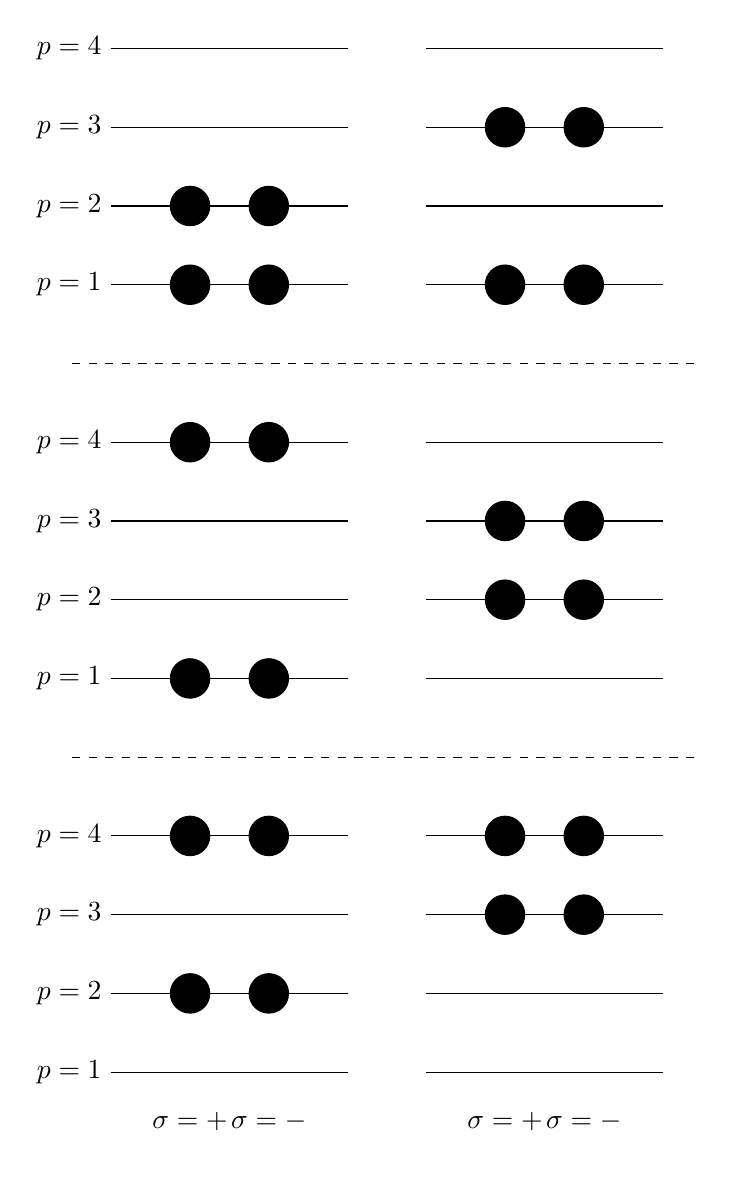
\begin{tikzpicture}
  
     \begin{scope}
      \foreach \i in {1,...,4}
      {
        \draw (-1,\i-1) node[anchor=east] {$p = \i$} --(2,\i-1);
      }
      \filldraw (0,0)  circle (0.25cm); 
      \filldraw (1,0)  circle (0.25cm);
      \filldraw (0,1) circle (0.25cm); \filldraw (1,1) circle (0.25cm);
      
      \draw[dashed](-1.5,-1) -- (2.5, -1);
      
    \end{scope}
    
    \begin{scope}[xshift=4cm]
      \foreach \i in {1,...,4}
      {
        \draw (-1,\i-1) --(2,\i-1);
      }
      \filldraw (0,0) circle (0.25cm); 
      \filldraw (1,0)  circle (0.25cm);
      \filldraw (0,2) circle (0.25cm); \filldraw (1,2) circle (0.25cm);
      
       \draw[dashed](-1.5,-1) -- (2.5, -1);
       
    \end{scope}   
    
    \begin{scope}[yshift=-5cm]
      \foreach \i in {1,...,4}
      {
        \draw (-1,\i-1) node[anchor=east] {$p = \i$} --(2,\i-1);
      }
      \filldraw (0,0) circle (0.25cm); 
      \filldraw (1,0)  circle (0.25cm);
      \filldraw (0,3) circle (0.25cm); \filldraw (1,3) circle (0.25cm);
     
	 \draw[dashed](-1.5,-1) -- (2.5, -1);     
     
    \end{scope}
   
    \begin{scope}[xshift=4cm, yshift=-5cm]
      \foreach \i in {1,...,4}
      {
        \draw (-1,\i-1) --(2,\i-1);
      }
      \filldraw (0,1) circle (0.25cm); \filldraw (1,1) circle (0.25cm);
      \filldraw (0,2) circle (0.25cm); \filldraw (1,2) circle (0.25cm);   
      
       \draw[dashed](-1.5,-1) -- (2.5, -1);
       
    \end{scope}
    
    \begin{scope}[yshift=-10cm]
      \foreach \i in {1,...,4}
      {
        \draw (-1,\i-1) node[anchor=east] {$p = \i$} --(2,\i-1);
      }
       \draw (0,0) node[anchor=north, inner sep=.5cm] {$\sigma=+$};
       \draw (1,0) node[anchor=north, inner sep=.5cm] {$\sigma=-$};
      \filldraw (0,1) circle (0.25cm); \filldraw (1,1) circle (0.25cm);
      \filldraw (0,3) circle (0.25cm); \filldraw (1,3) circle (0.25cm);  

	\end{scope}
	
	\begin{scope}[xshift=4cm, yshift=-10cm]
      \foreach \i in {1,...,4}
      {
        \draw (-1,\i-1)  --(2,\i-1);
      }
       \draw (0,0) node[anchor=north, inner sep=.5cm] {$\sigma=+$};
       \draw (1,0) node[anchor=north, inner sep=.5cm] {$\sigma=-$};
       \filldraw (0,2) circle (0.25cm); \filldraw (1,2) circle (0.25cm);
       \filldraw (0,3) circle (0.25cm); \filldraw (1,3) circle (0.25cm); 

	\end{scope}
	
  \end{tikzpicture}

\end{document}